\documentclass[12pt,usletter,fancy]{elegantbook}
\usepackage{tikz}
\usepackage{titlesec}
\usepackage{setspace}% spaces between lines
\usepackage{parskip}% spaces between paragraphs
\usepackage{xcolor}
\usepackage{tcolorbox}

\title{Genetic determinants of human phenotypes}
\subtitle{A study focusing on infectious diseases}

\author{Zhenhua Zhang}
\institute{University Medical Center Groningen}
%\date{\today}
%\version{4.1}
%\bioinfo{Bio}{Information}

%\extrainfo{Victory won\rq t come to us unless we go to it. }

%\logo{logo-blue.png}
\cover{cover.jpg}

\definecolor{mycolor}{RGB}{32,178,170}
\colorlet{coverlinecolor}{mycolor}

% Title font size, by package titlesec
\titleformat{\chapter}[display]{%
  \fontsize{35pt}{30pt}\bfseries}%
  {\textit{\color{black!50}{Chapter \thechapter}}}%
  {5pt}%
  {\color{cyan}{\chaptertitle}}

% Add a blank page
\def\blankpage{%
  \clearpage%
  \thispagestyle{empty}%
  \addtocounter{page}{-1}%
  \null%
\clearpage}

% Add a highlighted marks for sentence to add a ref on.
\newcommand{\reqref}[1][ref]{
  \colorbox{yellow}{\textbf{#1}}
}

% Set the line spacing to 1
\onehalfspacing

% Define a box and its style
% Reference https://texample.net/tikz/examples/boxes-with-text-and-math/
\tikzstyle{termbox} = [draw=black,fill=brown!20,very thick,rectangle,
  rounded corners,inner sep=10pt,inner ysep=20pt]
\tikzstyle{termtitle} = [fill=red!5,text=black]


\begin{document}
\maketitle
\frontmatter
% \tableofcontents
% \blankpage

\mainmatter

% \chapter*{Prepositions}
% \addcontentsline{toc}{chapter}{Prepositions}
% Content
% \blankpage

\chapter{General introduction}

\newpage
\section*{Genome-wide profiling of human molecular traits}
The human draft genome was released in 2001 by the Human Genome Project and Celera Corporation \textbf{[10.1038/nature03001]}, which have improved our understandings of its architecture and provided knowledge about the location and structure of genes.
However, the genetic diversity within and among human populations is required to biologically understand the whole picture of human body.
As a complement, the 1000 Genome Project demonstrated genetic variation among humans \textbf{[10.1038/nature11632]}.
It also supplied opportunities to identify genetic markers associated with traits of interest, especially diseases, using methods like genome-wide association studies (GWAS).
The genome-wide profile of biological molecule at large scale in human body is the corner-stone for the prosperity and success of GWAS.

\paragraph*{Profiling genetic molecules.}
The commonly used approaches are target-probe hybridization based technologies such as DNA microarray and NanoString \textbf{[10.1038/nbt1385]}.
These methods can identify various variants from small variants, such as single-nucleotide polymorphism (SNP) and short insertions/deletions (indel), to large variation, such as structural variation and copy number variants.
While, for rare variants, the innovation and development of next-generation sequencing (NGS) brought efficient and cost-effective methods to profile them for the whole exome (WES), genome (WGS), or transcriptome (WTS)\reqref.
These advancements promoted our understandings on genetic complexity and diversity in rare/complex diseases \reqref (e.g., cancers \reqref), microbe-host interactions \reqref, and human evolution \textbf{[10.1038/nrg3625]}.

\paragraph*{Profiling phenotypic molecular traits.}
% TODO: Joeri feels missing core message for current paragraph
The profile of human molecular traits that connect genotypes (i.e., genetic variants) and complex phenotypes (e.g., cancers) is a centre of attraction because studying these traits could aid to answer complex biological questions.
In the past decades, various molecular traits have been studied, such as gene expression (mRNA abundance) \reqref, chromatin accessibility \reqref, and latent viral genomes \reqref.
Many studies suggested molecular traits also resemble complex traits (e.g., height) in that the variation of the studied traits are attributed to heritable factors, environmental exposures, and their interplay\textbf{[10.1101/gr.176933.114]}.
These findings provoke questions like, how does the genome guide cells to produce, distribute, and consume different moleculars?
The comprehensive profiling of human molecular traits at diverse scale offers researchers chance to answer these questions by integrating different layers (i.e., multi-omics) of data to gain insights of complicated biological processes.

\paragraph*{Integration of multiple profiles of human molecular traits.}
To integrate multi-omics data, researchers combine profiles of molecular traits using general/advanced statistical and machine learning approaches, in which multi-omic integration studies encounter prosperity in the post-genome ara.
The integration ranges from personal multi-omics data to large cohort involving tens of thousands individuals.
At a personalized genome scale, integrative analyses of multi-omics profile, including genomic, transcriptomic, proteomic, and metabolomic measurements, suggested dynamics of molecular traits and diverse medical risks\textbf{[10.1016/j.cell.2012.02.009]}.
While, on large cohort scale, studies involving genomic and one/more molecular traits also broadened our knowledge about complex human phenotypes, e.g., common adult diseases \reqref and evolution of humans \reqref.

% TODO: a paragraph with a very brief summary what you told so far, then explain that you need all kinds of ingredients to start understanding (and ultimately, treating) complex (infectious) disease - 
% with each linking to a section below, ending with multi-omics integration of all these different layers of data, using the right models, to extract the knowledge etc.
% This way, all the sections below make sense.
Benefited from the omic techniques, researchers can profile genome-wide genotypes and molecular phenotypes at large scales, which supplies ingredients to understand mechanisms underlying complex diseases and ultimately treat them.
Statistically, the variations of a phenotype of interest can be partitioned based on nature-nurture model that is the corner-stone of GWAS.
Estimating the proportion of variance explained by each compartment (i.e., genetic and environmental factors) can help researchers prioritize factors that should be focused on.
Thus, the accurate estimation of genotypic proportion of the phenotype variations is essential to dissect genetic determinants of a phenotype, where both association and fine-mapping studies play important roles.
Additionally, the integration of multi-omic data also allows researchers to understand the biological mechanisms of human phenotypes from multiple aspects.


\section*{Phenotypic variation partition and association studies}
\paragraph*{Partition of phenotypic variation.}
The organisms' genome (e.g., human beings) contains huge amount of heritable information via its architecture and functions of genes.
The information determines the phenotype diversities and behaviors of the members in different populations.
However, an observed phenotype is also influenced by various environmental factors and their interactions with the heritable information.
Hence, the phenotype in a population can be statistically modeled through three components based on the nature-nurture model\reqref.
More are described in details \textbf{Box 1}. % TODO: use this in discussion.

\begin{figure}[h]
  \centering
  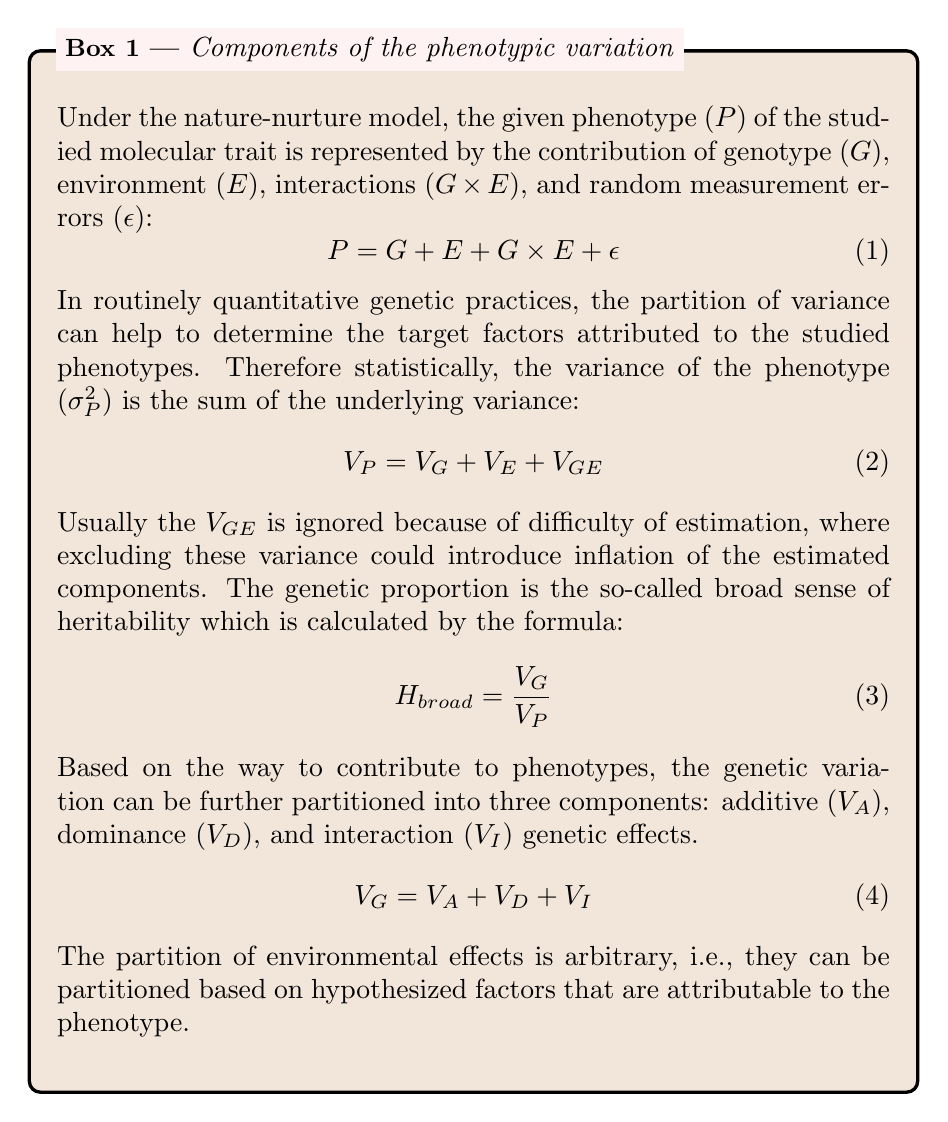
\begin{tikzpicture}
    \node [termbox] (box) {%
      \begin{minipage}{0.8725\textwidth}
        Under the nature-nurture model, the given phenotype ($P$) of the studied molecular trait is represented by the contribution of genotype ($G$), environment ($E$), interactions ($G \times E$), and random measurement errors ($\epsilon$):
        \begin{equation}
          P = G + E + G \times E + \epsilon
        \end{equation}
        In routinely quantitative genetic practices, the partition of variance can help to determine the target factors attributed to the studied phenotypes.
        Therefore statistically, the variance of the phenotype ($\sigma^2_P$) is the sum of the underlying variance:
        \begin{equation}
          V_P = V_G + V_E + V_{GE}
        \end{equation}
        Usually the $V_{GE}$ is ignored because of difficulty of estimation, where excluding these variance could introduce inflation of the estimated components.
        The genetic proportion is the so-called broad sense of heritability which is calculated by the formula:
        \begin{equation}
          H_{broad} = \frac{V_G}{V_P}
        \end{equation}
        Based on the way to contribute to phenotypes, the genetic variation can be further partitioned into three components: additive ($V_A$), dominance ($V_D$), and interaction ($V_I$) genetic effects.
        \begin{equation}
          V_G = V_A + V_D + V_I
        \end{equation}
        The partition of environmental effects is arbitrary, i.e., they can be partitioned based on hypothesized factors that are attributable to the phenotype.
      \end{minipage}}; %
      \node [termtitle, right=10pt] at (box.north west) {%
        \textbf{\small Box 1 |} \textit{Components of the phenotypic variation}};
  \end{tikzpicture}
  % \label{}
\end{figure}

\paragraph*{Genome-wide association studies.}
GWAS estimate the association between millions of genetic variants and phenotypes of interest (e.g., diseases and gene expression).
The test identifies the genetic contribution to the phenotypic variation regressing potential non-genetic factors and the underlying interactions, which can in turn bring insights of underlying biological mechanisms.
Since the very first GWAS work published in 2005 \textbf{[10.1126/science.1109557]}, more than 5,000 GWAS have been performed \textbf{[10.1038/s41588-019-0481-0]}
Regarding human beings, these GWAS pinpointed numerous genomic loci that are associated with up to \textcolor{red}{xxx} human traits, including gene expression traits\reqref, protein abundance\reqref, metabolites diversity\reqref, cell-type phenotypes\reqref, complex diseases\reqref, and other complex phenotypes\reqref.
The identified genomic loci gave insights in the underlying mechanisms of the studied phenotypes, for examples, type 2 diabetes\reqref and HIV-1 infection\reqref.
In GWAS studies, the phenotype of interest could be either continuous or discrete, which is modeled by logistic or linear models, respectively.
For continuous or quantitative phenotype, the identified genomic regions harboring genetic variation associated with quantitative traits are called quantitative trait loci (QTL).
Hence, genome-wide QTL analysis is an ideal way to identify genetic variants attributable to phenotypic variation.

\section*{Expression quantitative trait loci (eQTL)}
In routine GWAS practices, eQTL are usually used to interpret regulatory program by leveraging the gene expression profile and genetic variants at the genome-wide scale.
An eQTL is a genetic region or locus whose variation are statistically attributable to the expression of a gene.
The locus potentially modulates the gene expression via affecting RNA transcription activity, alternative splicing events, and the stability of RNA molecules.
Therefore, identifying eQTL for all genes or a panel of genes of interest is an ideal tool to discover novel genetic components that affect RNA abundance in given tissues or cell types\reqref.
The identified eQTL can be proximal (\textit{cis}-eQTL) or distal (\textit{trans}-eQTL) which depends on their distance to the regulated gene.
The \textit{cis}-eQTL which are proximal to the associated genes are commonly used to interpret and construct expression regulatory networks.
However, both \textit{cis}-eQTL and \textit{trans}-eQTL can only explain limited proportion of variations that are estimated for the phenotypes or traits of interest.
Given the small effect size of eQTL, large samples size is required to increase the statistical power to detect small effect size, especially for \textit{trans}-eQTLs.
Meta-analysis combines multiple summary statistics from different studies but working on the same material (e.g, tissue or cell type) to estimate small effect size of eQTLs.
Recently, a group of researchers performed a comprehensive meta-analysis using \textcolor{red}{xxx} eQTL summary statistics and identified a large set of eQTL regulating blood gene expression and suggested potential driving factors for complex phenotypes \textbf{[10.1038/s41588-021-00913-z]}.

\section*{GWAS for infectious diseases}
The causes of infectious diseases are pathogens including virus, bacteria, fungi and parasites.
The innovation and discovery of antibiotic like penicillins almost eliminated mortal threats of bacterial infections.
However, many infectious disease, such as viral infection by human immunodeficiency virus (HIV) and severe acute respiratory syndrome coronavirus (SARS), are still hazard to the public health.
Infections provoke host immune response and could be as critical as life-threatening.
When the host's immune defence system fails or compromise, the disease symptoms may emerge and develop, where the final outcome may be deadly.
Due to the strong heritability of susceptibility to immune-mediated diseases like fatal infections, many GWAS on infectious diseases identified host-side genetic factors attributable to the diseases symptoms (e.g., acquisition, severity and latency).

\paragraph*{Acquired immunodeficiency syndrome (AIDS).}
HIV causes AIDS, which is characterized by noticeable heterogeneity in terms of susceptibility and disease progression rates after infection.
In 2007, the first reported GWAS on AIDS was published in which the HIV RNA viral loads at the disease set-point were associated with genome-wide SNPs\textbf{[10.1126/science.1143767]}.
Since then, many GWAS focusing on different AIDS phenotypes were performed and identified genetic loci (e.g., \textit{HCP5} and \textit{HLA-C} loci) associated with AIDS symptoms including HIV susceptibility\textbf{[10.1097/QAD.0b013e328343817b;10.1128/JVI.01499-12]}, disease progression \reqref, viral load control \textbf{[10.1126/science.1143767]}, HIV acquisition \textbf{[10.1371/journal.ppat.1003515]}, mother-to-child transmission \textbf{[10.1186/gm138]}, etc.
Moreover, HIV-1 acquisition was polygenic and heritable which was suggested by a GWAS meta-analysis \textbf{[10.1038/s41598-020-59256-0]}.

\paragraph*{Coronavirus disease 2019 (COVID-19).}
Since the end of 2019, the COVID-19 pandemic has brought about hundreds of millions confirmed cases and millions reported death according to the COVID-19 Dashboard by the Center for Systems Science and Engineering at Johns Hopkins University\reqref.
To combat this deadly disease, to date, several large-scale GWAS identified genetic variants associated with the severity of COVID-19\textbf{[10.1056/NEJMoa2020283; 10.1038/s41586-020-03065-y;10.1038/s41586-021-03767-x;10.1038/s41588-021-00854-7]}.
The identified genetic loci revealed underlying mechanisms of host anti-virus defence and organ damage caused by inflammation in COVID-19.
This in turn provided new drug-targets for future prevention and treatment.

\section*{Allele-specific analysis}
A useful technique for finding cis-regulated gene expression variants that underpin phenotypic differences across individuals is allele-specific analysis, which measures the relative difference of two alleles in diploid organisms, e.g., allele-specific expression \textbf{[10.1371/journal.pgen.1008786]}.
For diploid organisms, the genetic and epigenetic (partially) characteristics of two alleles are inherited from parents who usually consist of distinct genetic and epigenetic information.
The difference between two parental alleles are critical for the diversities of offspring's phenotypes.
Thus, quantification of the difference can give insights in the underlying mechanisms of regulating program.
Studies involving allele-specific analysis for open chromatin (ASoC), expression (ASE), and methylation (ASM) reveal complex regulatory networks underlying the studied traits\reqref.
The allele-specific analysis and potential application are illustrated in \textbf{Figure \ref{fig:example-image-a}}.

\paragraph*{ASoC analysis.} The gene expression in eukaryotic organisms is modulated at different stages, including chromatin opening, basal transcription factors (TF) binding to core promoter forming TF-DNA complex, and then the polymerase biding to TF-DNA complex.
However, in most cases, the promoter regions interact with other local or distal sequences (e.g., enhancers, insulators, and silencers).
Enhancer sequences guide the formation of activator complexes which determine the activation of a promoter in a cell-type specific or non-specific manner.
Interactions between enhancers and promoters a usually proximal (up to 100bp), but also can be distal up to tens of kilobases\reqref.
The chromatin is usually closed and commonly play a negative regulatory role, thus the regulation of chromatin openness is crucial to manipulate gene expression in all cell types or specific cell types.
Therefore, by assessing the allelic accessibility of chromatin at heterozygous genetic variants (e.g., SNPs), regulating program due to chromatin remodeling or modification can be identified.
For instance, by identifying ASoC SNPs in pluripotent stem cell-derive neurons, the study highlighted functional mechanisms of noncoding risk variants in development of neurons \textbf{[10.1126/science.aay3983]}.

\paragraph*{ASM analysis}
The demethylation of the promoter regions (5-prime end of the gene) can be vital for transcription initiation, which is a reversible epigenetic regulating scheme.
In genomes of diploid mammalian, the well-described ASM are imprinted regions and X-chromosome inactivation in females, while, additionally, heterozygous SNPs of ASM displayed a mild frequency in pluripotent human cells and a distinct ASM profiles across cell types were observed \textbf{[10.1101/gr.104695.109]}, which suggests genetic contribution to epigenome.
Thus, identifying ASM SNPs could be an useful methods to localize regulatory SNPs at the post-GWAS stage \textbf{[10.1186/s13059-020-02059-3]}.

\paragraph*{ASE analysis.}
Theoretically, ASE is the result of ASoC, ASM, or genetic regulations.
Recent studies suggested ASE plays roles in disease etiology, such as autism \textbf{[10.1038/s41593-019-0461-9]} and colorectal cancer\textbf{[10.1126/science.1159397]}.
In practice, researchers determine the allelic imbalance of RNA abundance from the same transcript in diploid species (e.g., human beings) by RNA sequencing, where heterozygous genetic markers (e.g., SNPs) are required to distinguish one allele from the other.
The well-developed large-scale profiling techniques for transcriptome and genomic variants enable researchers to identify ASE at genome-wide and large cohort scale.
Together with clinical and demographic information, ASE analysis is an powerful approach to pinpoint potential biological mechanisms, e.g., regulatory elements in proximal to the genes involving in phenotypes of interest.
Moreover, ASE also works as a complementary for QTL analysis in fine-mapping studies to attribute genetic variants to phenotypes of interest\reqref.

\begin{figure}[h]
  \centering
  \includegraphics[width=\textwidth,height=5cm]{example-image-a}
  \vspace*{0.2cm}
  \caption{Allelic analysis schemes}
  \label{fig:example-image-a}
\end{figure}

\section*{Multi-omics integration in post-genome era}
The integration of multiple layer of omics data aims to holistically understand complex biological processes using molecular variations from different levels data including genome, epigenome, transcriptome, proteome, and metabolome.
Together with phenotypic data, e.g., clinical and demographic information, integrative analysis of multi-omics is a promising approach to interpret biological mechanisms of complex phenotypes \textbf{[10.1093/bib/bbx066]} and likely to innovate novel diagnostic schemes and therapeutic tactics \textbf{[10.1142/9789814583220\_0013; 10.1093/bib/bbx066]}.
Base on the way to combine different omics data, there are two schemes to integrate multi-omics data: multi-stages and multi-modal scheme (\textbf{Figure \ref{fig:example-image-b}}).

\begin{figure}[h]
  \centering
  % \includegraphics[width=\textwidth]{chapter_1_figure_1.png}
  \includegraphics[width=\textwidth,height=5cm]{example-image-b}
  \vspace*{0.2cm}
  \caption{Schemes of multi-omic integrative analysis.}
  % \label{fig:chapter_1_figure_1}
  \label{fig:example-image-b}
\end{figure}

\paragraph*{Central dogma centered multi-stages scheme.}
In molecular biology, the central dogma (\textbf{Box 2}) describes a macroscopic flow which transmits genetic information from genome to phenotypes across multiple biological stages (multi-stage).
The biological multi-stage nature allows researchers to integrate multi-omics data using a divided-conquer strategy.
Concretely, the analysis is divided into isolated scopes, both biologically and technically.
Then, for each scope, proper statistical analysis is performed independently and main findings are prepared in a compatible format across all scopes.
By combining the findings, the results are interpreted in respect to the information flow under central dogma hypothesis.
One frequently used method is the combination of various QTL from transcriptome (eQTL), epigenome (methylation QTL or methQTL), proteome (protein QTL or pQTL), and metabolome (metabolites QTL or mQTL).
The other approach is the integration through functional and pathway informations which are reviewed and consolidated by experts and initiatives, e.g., Gene Ontology (GO) Consortium\reqref and Kyoto Encyclopedia of Genes and Genomes (KEGG)\reqref.

\paragraph*{Multi-modal centered scheme.}
In contrast to the divided-conquer strategy in multi-stages approaches, the multi-modal centered scheme analyzes all layers of omics data simultaneously.
The underlying hypothesis is that each type of omics data is a snapshot at a specific perspective.
The proper combination of all perspectives and subsequent abstracts by decent statistical and machine learning techniques can give insights into the underlying biological mechanisms.
In this scheme, the ultimate goal is to build a model or an ensemble model from all measured omic data.
The data reprocessing and organization before the model construction could be scoped into concatenation-based, transformation-based, and multi-model-based methods\textbf{[10.1038/nrg3868]}.
E.g., For transformation-based methods, a kernel-based integrative analysis was used to build model which predicts protein functions via different type of features \textbf{[10.1093/bioinformatics/bth294]}.

\begin{figure}[h]
  \centering
  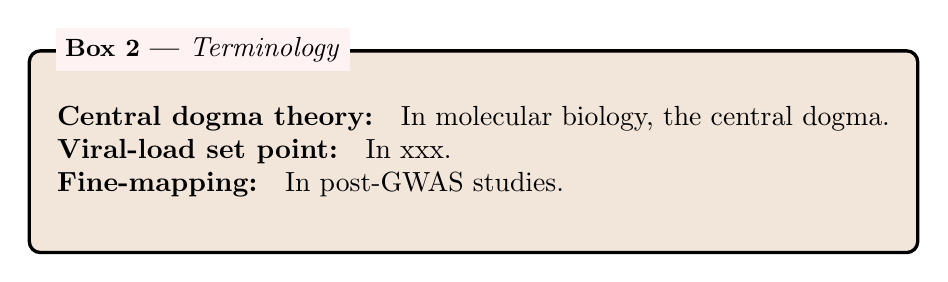
\begin{tikzpicture}
    \node [termbox] (box) {%
      \begin{minipage}{0.8725\textwidth}
        \paragraph*{Central dogma theory:} In molecular biology, the central dogma.
        \paragraph*{Viral-load set point:} In xxx.
        \paragraph*{Fine-mapping:} In post-GWAS studies.
      \end{minipage}}; %
      \node [termtitle, right=10pt] at (box.north west) {%
        \textbf{\small Box 2 |} \textit{Terminology}};
  \end{tikzpicture}
\end{figure}

\section*{Purpose and outline of the current thesis}
This thesis aims to understand the association between genetic architecture and various human molecular traits genome-widely.
However, due to the complicated relations between human genotypes and phenotypes, this work will investigate and answer a number of important open questions that are essential in completing the full picture.

\paragraph*{The Chapter 1}(the current chapter) is a general introduction and a summary for the whole thesis.
\paragraph*{The Chapter 2} is a study to estimate the feasibility to predict the ASE effects from genetic variants (SNPs) using ML methods.
\paragraph*{The Chapter 3}...
\paragraph*{The Chapter 4}...
\paragraph*{The Chapter 5}...
\paragraph*{The Chapter 6}...
\paragraph*{The Chapter 7}...

% \chapter{ASE prediction}
% \section*{Abstract}
% \paragraph*{Backgrounds:}
% \paragraph*{Methods:}
% \paragraph*{Results:}
% \paragraph*{Conclusion:}
% 
% \section*{Background}
% \section*{Results}
% \section*{Summary and conclusion}
% \section*{Methods}
% 
% \chapter{ASE deep learning}
% 
% \chapter{COVID-19 MHH50}
% 
% \chapter{HIV reservoir QTL}
% 
% \chapter{CCR5 expression QTL}
% 
% \chapter{Summary and general discussion}
% 
% \chapter*{Dutch summary (Netherlandse samenvatting)}
% \addcontentsline{toc}{chapter}{Netherlandse samenvatting}
% 
% \chapter*{Acknowledgements}
% \addcontentsline{toc}{chapter}{Acknowledgements}
% 
% \appendix
% \chapter*{Appendices}
% \addcontentsline{toc}{chapter}{Appendices}
% \section*{CV -- Z. Zhang}
% \addcontentsline{toc}{section}{CV -- Z. Zhang}
% \section*{Publication list}
% \addcontentsline{toc}{section}{Publication list}

\end{document}

% vim: set tw=500:
